\chapter{Penalty Hamiltonians for state verification}
\label{chap:ghz}

In this chapter, we propose and study a new method to estimate the fidelity of Clifford states. Primarily we focus on the Greenberger--Horne--Zeilinger (GHZ) state, as preparation of this state with high fidelity is an important benchmark for quantum hardware. We will start by reviewing the existing techniques tailored to verification of the GHZ state. Then we will introduce our proposal based on measuring the expected value of a certain Hamiltonian constructed using the description of the quantum circuit. Finally, we will present our numerical experiments and discuss their results.

\section{Background}

There are various methods to characterize quantum devices. The choice of a technique depends on the information we need to obtain, the amount of resources we can spend, and the assumptions made about the system of interest. The most dierct method to characterize a state prepared by the device is called quantum tomography~\cite{dariano_quantum_2003,straupe_adaptive_2016}. In quantum tomography, one repeatedly prepares a state of interest and measures it in different bases to completely reconstruct its density matrix. Unfortunately, full quantum tomography takes exponential time in the number of qubits, so it is only applicable to small systems and gates. Another recently proposed method, shadow tomography~\cite{aaronson_shadow_2018,huang_predicting_2020,koh_classical_2020}, enables the estimation functions linear in the density matrix $\rho$ without characterizing the state completely. Average properties of quantum circuits prepared by the device can also be inferred using a process called randomized benchmarking~\cite{magesan_robust_2011-1,knill_randomized_2008}.

One more metric for quantum computers is the size of the largest entangled state it can reliably prepare. In what follows we focus on the Greenberger--Horne--Zeilinger (GHZ) state $\ket{\Psi} = \frac{1}{\sqrt{2}} (\ket{0...0} + \ket{1...1})$. This state is a textbook example of a quantum state exhibiting genuine multipartite entanglement, meaning that there is no bipartition of qubits that would make this state separable. In addition, any state whose fidelity with the GHZ state above $1/2$ is guaranteed to be entangled (this is true even for mixed states)~\cite{sackett_experimental_2000}. Because of that, the fidelity of $1/2$ is used as a threshold benchmark for real quantum devices. Due to the simple form of the GHZ state, it is possible to estimate its fidelity without resorting to full state tomography. In the following subsection, we describe the existing techniques developed specifically for the GHZ state.

\subsection{Fidelity measurement techniques for the GHZ state}

\subsubsection{Parity oscillations}

A common technique to evaluate the fidelity of a quantum state with the GHZ state is based on measuring the \emph{parity oscillations} \cite{sackett_experimental_2000,leibfried_toward_2004,leibfried_creation_2005,monz_14-qubit_2011,song_observation_2019,omran_generation_2019}. 
The diagonal components $\rho_{0...0, 0...0}$ and $\rho_{1...1, 1...1}$ are measured in the computational basis. If we measure the off-diagonal components $\rho_{0...0, 1...1}$ and $\rho_{1...1, 0...0}$ (which are complex conjugates of each other), we can calculate the fidelity. The latter is usually expressed as a sum of two unknown values, called population $P$ and coherence $C$:
\begin{equation}
    \label{eq:f_is_p_plus_c}
    F = \frac{1}{2} (P + C).
\end{equation}
Here $P = \rho_{0...0, 0...0} + \rho_{1...1, 1...1}$, and 
$C = 2 |\rho_{1...1, 0...0}|$. 
\begin{remark}
    Strictly speaking, the fidelity is equal to $\frac{1}{2} (P + 2 \operatorname{Re} \rho_{1...1, 0...0})$. However, if one only cares about the multipartite entanglement, then one can estimate fidelity with the closest state of the type $\frac{1}{\sqrt{2}} (\ket{0...0} + e^{\rmi \gamma}\ket{1...1})$. In this case, the estimate is given by Eq.~(\ref{eq:f_is_p_plus_c}).
\end{remark}
The population is straightforward to measure. Evaluating coherence, on the other hand, requires a more complicated setup. The implementation is different depending on the platform, but the overall idea is to induce a phase difference $\varphi$ between the components of the GHZ state, and then measure an observable that would be sensitive to this phase difference. 



The method employed in trapped-ion processors  consists in applying a local unitary gate $U = e^{-\rmi \frac{\pi}{4} (\cos \varphi X + \sin \varphi Y)}$ to every qubit. Then, the state is measured in the $Z$ basis. The value of interest is the parity, i.e.~the ratio of measurements with an even number of ones minus the ratio of measurements with an odd number of ones. Effectively, this means measuring the expected value of $Z^{\otimes n}$. If we denote $\rho_{0...0, 1...1} = re^{i \gamma}$, then the value of parity will have an oscillating component equal to $2r \cos(n \varphi - \gamma)$. Fitting the parity with a sine curve and extracting $\rho$ and $\gamma$ enables the calculation of fidelity.



\subsubsection{Multiple quantum coherence}

The value of $C$ can also be measured by method of multiple quantum coherences (MQC) \cite{wei_verifying_2020}. Excluding the technical error-mitigating steps, the method goes as follows:
\begin{enumerate}
    \item Prepare the GHZ state;
    % \item Apply a $X$ gate to every qubit;
    \item Apply a $Z$ rotation with angle $\varphi$ to each qubit;
    \item Unprepare the GHZ state, i.e.~apply the entangling gates in reverse order;
    \item Measure the first qubit in the $Z$ basis. Record the  probability of measuring $\ket{0...0}$ as the overlap signal $S_\varphi$.
\end{enumerate}

The steps 1-4 must be repeated for $\varphi = \frac{\pi j}{n+1}$ for $j = 0, 1, ..., 2n+1$. Finally, by computing the Fourier transform of $S_\varphi$ and taking the highest-frequency component $I_n$, we can calculate the coherence as $C = 2 \sqrt{I_n}$. 

To mitigate errors, the authors also apply an $X$ gate to every qubit after step one. For a perfect GHZ state, this step does nothing. However, in experimental conditions there is a coherent error that results in the state drifting from the desired position. The application of $X$ gates effectively reverses the direction of the drift, enabling better overall coherence of the state for a while. This is analogous to the spin echo effect~\cite{hahn_spin_1950}.

It is interesting to compare MQC to parity oscillations. An obvious downside is that MQC requires the circuit to be twice as long. Another disadvantage is that, strictly speaking, the method depends on certain assumptions about the noise in the device~\cite{garttner_relating_2018}. However, there are advantages as well. First, MQC enables the aforementioned error mitigation by $\pi$-pulses. Second, MQC is easier to correct for readout errors \cite{wei_verifying_2020}. In MQC, the ideal measurement contains only the strings $00...0$ and $10...0$, as opposed to parity oscillations, where all strings should be expected.

The current record of preparing the GHZ state for 27 qubits \cite{mooney_generation_2021} uses the MQC technique for verification.

% How do you estimate fidelity with RB? Can you at least do it on average?

\section{Stability lemma and telescope construction}

Quantum states can be encoded into ground states of local Hamiltonians. If one has such a Hamiltonian with a unique ground state $\ket{\psi}$, then measuring its energy with respect to the state $\ket{\phi}$ enables us to estimate the fidelity of $|\braket{\phi}{\psi}|^2$ via the following lemma, extending the stability lemma from \cite{biamonte_universal_2021}.

\begin{proposition}[Stability lemma]
    \label{prop:stability}
    Let $H$ be a Hamiltonian with eigenvalues $0 = \lambda_0 < \Delta = \lambda_1 \leq \lambda_2 \leq ... \leq \lambda_{\mathrm{max}}$ and corresponding eigenvectors $\ket{\lambda_i}$. Let $\rho$ be a density operator such that $E = \Tr \rho H \leq \Delta$. Then
    \begin{equation}
        \label{eq:stability_lemma}
        1 - \frac{E}{\Delta} 
        \leq \bra{\lambda_0} \rho \ket{\lambda_0}
        \leq 1 - \frac{E}{\lambda_{\mathrm{max}}}.
    \end{equation}
\end{proposition}
\begin{proof}
    The trace of $\rho$ is equal to one, so the desired fidelity is a function of all other diagonal elements:
    \begin{equation}
        \label{eq:stability_proof}
        \rho_{00} = \bra{\lambda_0} \rho \ket{\lambda_0} = 1 - \sum_{i > 0} \rho_{ii}.
    \end{equation}
    The condition that $E$ is below the gap lets us find an upper bound on $\sum_{i > 0} \rho_{ii}$:
    \begin{equation}
        \sum_{i > 0} \rho_{ii} = \frac{1}{\Delta} \sum_{i > 0} \rho_{ii} \Delta \leq \frac{1}{\Delta} \sum_{i > 0} \rho_{ii} \lambda_{i} = \frac{E}{\Delta}.
    \end{equation}
    Another bound can be obtained in a similar fashion:
    \begin{equation}
        \sum_{i > 0} \rho_{ii} = \frac{1}{\lambda_{\text{max}}} \sum_{i > 0} \rho_{ii} \lambda_{\text{max}} \geq \frac{1}{\lambda_{\text{max}}} \sum_{i > 0} \rho_{ii} \lambda_{i} = \frac{E}{\lambda_{\text{max}}}.
    \end{equation}
    Substituting these two bounds into (\ref{eq:stability_proof}) yields the desired bounds.
\end{proof}

So, if we want to estimate the fidelity of quantum state $\rho$ with respect to the pure state $\ket{\psi}$ that was intended to be prepared, what we can do is find a Hamiltonian that contains that state in its ground space, measure the expected value of said Hamiltonian, and then find the bounds using Lemma~\ref{prop:stability}. In general, it is not clear how --- and whether it is possible --- to construct such a Hamiltonian so that it contains a polynomial number of Pauli terms, although the state can be encoded in the ground state of a local Hamiltonian using ancilla qubits~\cite{kitaev_classical_2002,biamonte_universal_2021}. However, for a class of states called Clifford states the task of finding a good Hamiltonian is rather easy. To explain the construction, we first define the Clifford group.

\begin{definition}[Clifford group]
    The \emph{Clifford group} $\mathcal{C} \subset \mc{U}(2^n)$ consists of operators $U$ such that their action by conjugation maps Pauli strings to Pauli strings. In other words, the Clifford group is the normalizer of the Pauli group. A quantum state of the type $U \ket{0...0}$ for $U \in \mc{C}$ is called a \emph{Clifford state}.
\end{definition}

What makes this group relevant is that it includes a large class of quantum circuits called \emph{Clifford circuits}.

\begin{proposition}[\cite{nielsen_quantum_2010}]
    The Clifford group is generated by the following gates, called respectively Hadamard, Phase and CNOT:
    \begin{equation}
        H = \frac{1}{\sqrt{2}}\begin{pmatrix}
            1 & 1 \\ 1 & -1
        \end{pmatrix},
        \quad
        P = \begin{pmatrix}
            1 & 0 \\ 0 & \rmi
        \end{pmatrix},
        \quad
        CNOT = \begin{pmatrix}
            1 & 0 & 0 & 0 \\ 
            0 & 1 & 0 & 0 \\ 
            0 & 0 & 0 & 1 \\ 
            0 & 0 & 1 & 0 
        \end{pmatrix}.
    \end{equation}
\end{proposition}

These gates act by conjugation on Pauli strings as follows (we write here only the action on generators of the Pauli group): 

\begin{align}
    H&: X \mapsto Z, Z \mapsto X \\
    P&: X \mapsto Y, Z \mapsto Z \\
    CNOT&: XI \mapsto XX, IX \mapsto IX, ZI \mapsto ZI, IZ \mapsto ZZ
\end{align}

The key fact about the Clifford group is that Clifford circuits can be simulated classically in polynomial time \cite{gottesman_heisenberg_1998,aaronson_improved_2004}. The idea is to keep track not of the Clifford state itself, but of the Pauli strings that stabilize it. The stabilizer subgroup of any Clifford state contains $2^n$ Pauli strings, however it is sufficient to consider just $n$ generating Pauli strings. With each gate, we act on them by conjugation and again receive Pauli strings. Ref.~\cite{aaronson_improved_2004} develops a more advanced algorithm to calculate the stabilizers and to evaluate the observables w.r.t.~the Clifford state.

The telscoping construction uses the idea of Clifford stabilizers. First we consider the state $\ket{0...0}$. Its stabilizer subgroup is generated by one-local Pauli strings $Z_i$. It is straightforward to check that the following Hamiltonian has $\ket{0...0}$ as the only ground state:

\begin{equation}
    H_0 = -\sum_{i = 1}^n Z_i + n \id
\end{equation}

Here the constant operator is added to shift the spectrum of the Hamiltonian, so that the ground state has zero energy. For any unitary $U$, it is true that the state $U \ket{0...0}$ is the unique ground state of the Hamiltonian $U H_0 U^\dagger$. When $U$ is a Clifford circuit, $H_0$ consists of $(n+1)$ Pauli strings. Thus we define this to be the \emph{telescope Hamiltonian} for the given Clifford circuit.

\begin{definition}
    A \emph{telescope Hamiltonian} for a Clifford circuit $U_L ... U_1$ is the following Hamiltonian:
    \begin{equation}
        \label{eq:telescope}
        H_{\text{tele}} = U_L ... U_1 H_0 U_1^\dagger ... U_L^\dagger.
    \end{equation}
\end{definition}

In particular, we can explicitly find the telescope Hamiltonian for the GHZ state. Recall that a standard circuit for preparing it looks like this:
\begin{equation*}
    \Qcircuit @C=1.0em @R=1.0em {
       & \lstick{\ket{0}} & \gate{H} & \ctrl{1} 
       & \qw & \qw & \qw  & \qw
       \\
       & \lstick{\ket{0}} & \qw & \targ 
       & \ctrl{1} & \qw & \qw & \qw
       \\
       & \lstick{\ket{0}} & \qw & \qw
       & \targ & \ctrl{1} & \qw & \qw
       \\
       & \lstick{\ket{0}} & \qw & \qw
       & \qw & \targ & \qw & \qw
       \\ & \ & \ & \ & ... & \ 
       \\
       & \lstick{\ket{0}} & \qw & \qw
       & \qw & \qw & \ctrl{1} & \qw
       \\
       & \lstick{\ket{0}} & \qw & \qw
       & \qw  & \qw & \targ & \qw
    }
\end{equation*}
By acting with Clifford gates by conjugation on $H_0$, we arrive to the following Hamiltonian:

\begin{equation}
    H = -\sum_{i=1}^{n-1} Z_i Z_{i+1} - X^{\otimes n} + n.
\end{equation}

Its only ground state is the GHZ state, and the constant term sets the ground state energy to zero. Thus, we can estimate the fidelity of a candidate GHZ state. Using Lemma~\ref{prop:stability}, we obtain
\begin{equation}
    1 - \frac{\langle H_\mathrm{tele} \rangle}{2}  \leq F \leq 1 - \frac{\langle H_\mathrm{tele} \rangle}{2n}.
\end{equation}
Evaluating this energy requires two series of measurements: in the $Z$ basis and in the $X$ basis. Unlike the parity oscillations technique, there is no need to scan through different values of $\varphi$.

\section{Numerical experiments}

\subsection{Local depolarizing errors}

It is interesting to compare the scaling of errors for different fidelity estimation techniques, e.g.~as a function of the number of shots and of the number of qubits. There is a certain difficulty with that: the results also heavily depend on the noise model. In the following, we adopt a simple noise model. We assume that every single-qubit (two-qubit) gate is followed by a single-qubit (two-qubit) depolarizing noise channel with depolarization probability $p_1$ ($p_2$).

In discussion of errors, we need to stress that we can estimate random errors, but not necessarily systematic errors. For example, the parity oscillation method requires us to measure qubits in the $X$ basis, but this means applying an extra Hadamard gate to every qubit before measurement. As a result, in the depolarizing noise model, this leads to a systematic underestimation of coherence. Random errors are, on the other hand, analyzable using the measurement statistics as usual.

We estimate the random errors of population and telescopic bounds by standard techniques. That is, the standard error of the mean is the square root of the sample variance divided by the number of measurements $\sqrt{N_{shots}}$. The coherence measurements are more complicated. In the case of parity oscillations, the coherence is a parameter obtained from a curve fit, while for MQC the coherence is obtained as a specific Fourier coefficient of the data. For these two estimates, the standard error is calculated by parametrized bootstrap resampling (using $B=100$ bootstraps). More specifically, for each value of $\varphi$, we treat the measurement result as having two outcomes (''even'' or ''odd'' for parity, ''0'' or ''1'' for multiple quantum coherences). Then, we infer the success probability $q_\varphi$ for each point. Then, we prepare the bootstrap measurement data by sampling from the binomial distributions $\mathcal{B}(q_\varphi, N_{shots})$. Finally, we obtain the coherence estimate. Repeating this $B$ times yields $B$ bootstrap coherence estimates $\hat{C}_i$. The variance of these coherences is our estimate of the standard error.

Figure \ref{fig:fidelity_terms} shows the behavior of the estimates of different terms as we increase the number of shots that are used in the experiment. The experiment was conducted for $n=8$ qubits with the depolarizing noise model ($p_1 = 0.001, p_2 = 0.01$). The telescope bounds in this case are substantially looser than the estimates from the other techniques, except for the small shot counts.

Figure \ref{fig:errors_as_nq} shows the dependence of the standard error on the number of qubits $n$. The number of shots per point was fixed at $2^{15}$. Surprisingly, the multiple quantum coherences method appears to show the worst scaling of the error, while the parity oscillations method gives an almost constant random error. The telescopic lower bound has a random error steadily growing with the size of the system. The upper bound behaves as $1/N$ by construction, so its error appears to decrease.

\begin{figure}
    \centering
    \includegraphics[width=0.7\textwidth]{figures/fidelity_terms_8_qubits_1645796806.eps}
    \caption{Sample size dependence of telescope lower ($\blacktriangle$) and upper ($\blacktriangledown$) bounds, population estimate ($\blacksquare$), and coherence estimates using parity oscillations ($\bullet$) and MQC ($\hexagofill$). Vertical lines denote one standard error.}
    \label{fig:fidelity_terms}
\end{figure}

Finally, Figure \ref{fig:errors_as_nshots} shows the dependence of random errors on the number of shots, while everything else is fixed. As expected, for all methods, the error behaves as $1/\sqrt{N_{shots}}$.

\begin{figure}
    \centering
    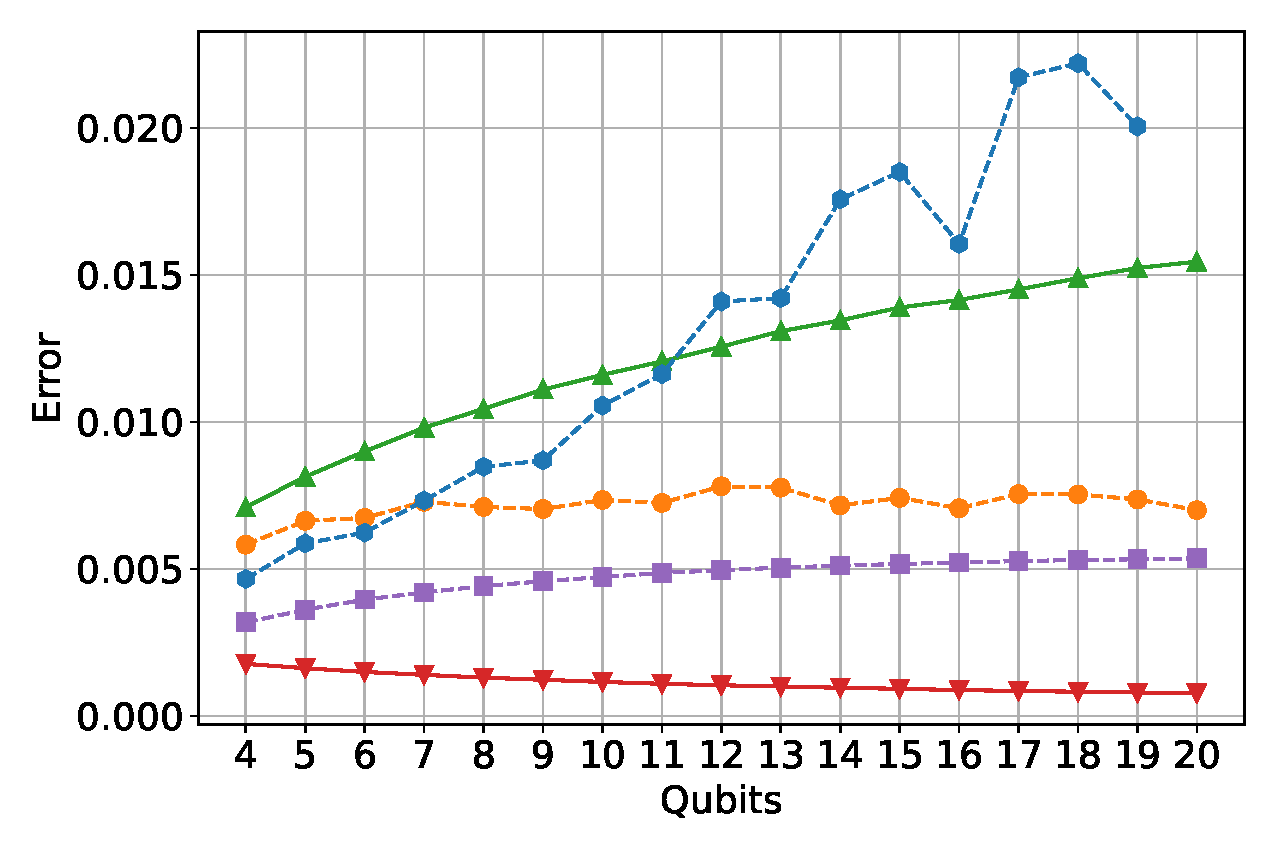
\includegraphics[width=0.7\textwidth]{figures/errors_as_nq_1645806507.eps}
    \caption{Estimates of random errors of telescope lower ($\blacktriangle$) and upper ($\blacktriangledown$) bounds, population estimate ($\blacksquare$), and coherence estimates using parity oscillations ($\bullet$) and MQC ($\hexagofill$). The errors for population and telescopic bounds are estimated by taking the standard error of the mean, the coherence errors are estimated by parametrized bootstrap resampling (see main text).}
    \label{fig:errors_as_nq}
\end{figure}

\begin{figure}
    \centering
    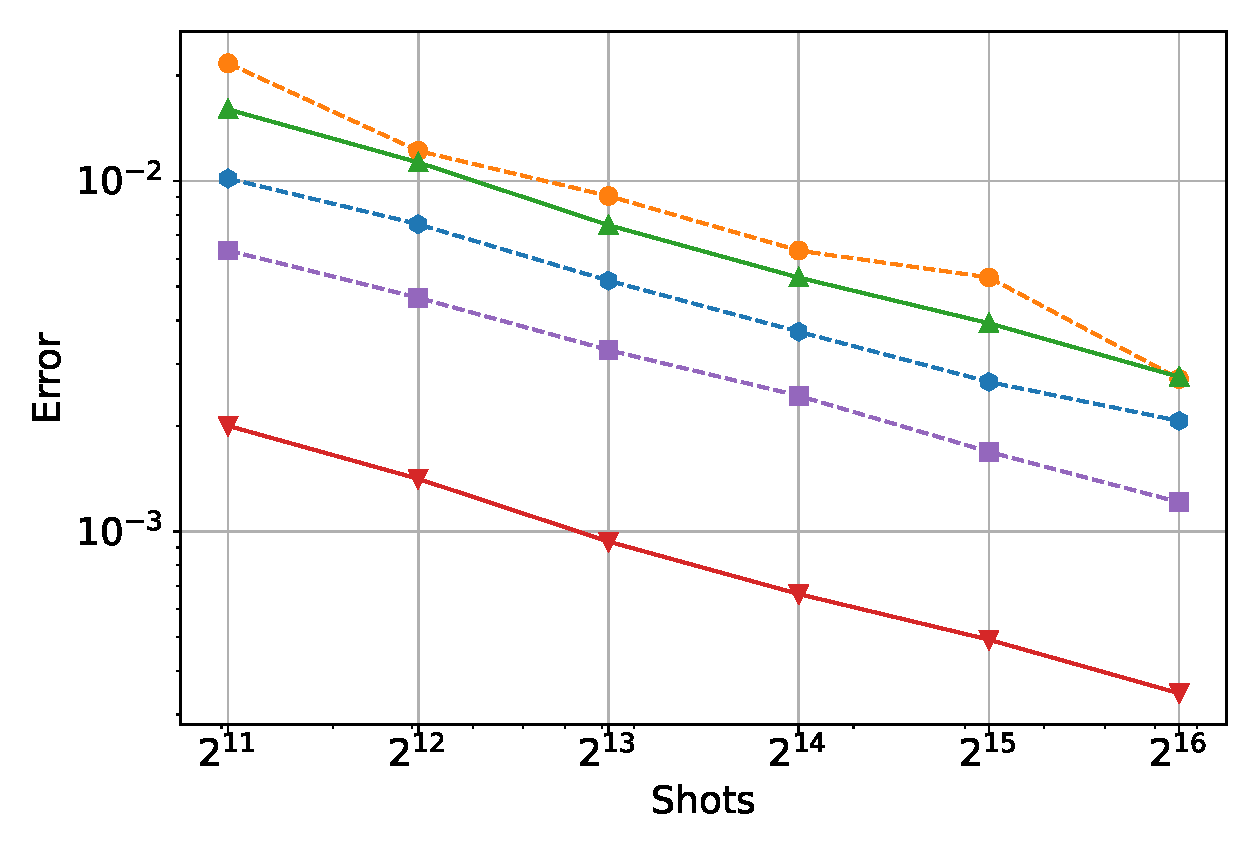
\includegraphics[width=0.7\textwidth]{figures/errors_8_qubits_1645796806.eps}
    \caption{Sample size dependence of the standard errors in the terms comprising different fidelity estimates. The markers match those in Fig.~\ref{fig:fidelity_terms}.}
    \label{fig:errors_as_nshots}
\end{figure}

\subsection{Global depolarizing error}

We analyzed the behavior of all three methods for the following family of states:
\begin{equation}
    \label{eq:partially_mixed}
    \rho(\alpha) = (1-\alpha) \ket{\Phi} \bra{\Phi} + \frac{\alpha}{2^n} \id.
\end{equation}
Here $\ket{\Phi}$ is the GHZ state. For that density matrix, we can exactly calculate the fidelity and the bounds provided by the telescope construction. The fidelity with the clean GHZ state is equal to 
\begin{equation}
    F = \bra{\Phi} \rho \ket{\Phi} = 1 - \alpha + \frac{\alpha}{2^n}.
\end{equation}
The energy of this state with respect to the telescope Hamiltonian is equal to $\frac{\alpha}{2^n} \Tr H = n \alpha$. Hence, the fidelity bounds provided by Proposition~\ref{prop:stability} are as follows:
\begin{equation}
    1 - \frac{n \alpha}{2} \leq F \leq 1 - \frac{\alpha}{2}.
\end{equation}
The lower bound deteriorates with the increase of $n$, becoming completely uninfomative at $\alpha = 2/n$. The upper bound, on the other hand, does not depend on $n$.

All three methods were tested numerically for determining the fidelity of $\rho$. In case of parity oscillations and multiple quantum coherences techniques, the simulation is somewhat artifical. The matter is that both of these techniques are substantially affected by measurement errors, which are not accounted for in this model. Instead, the methods receive the state $\rho$, then perform all necessary actions with perfect fidelity.

For every tested value of $\alpha$, 1000 measurements were allocated for measuring coherence (or, for the telescope, the expected value of $X^{\otimes n}$), and 1000 measurements were allocated for measuring population (respectively, the expectations of $Z_i Z_{i+1}$). For coherence measurements, the values of $\varphi$ were equal to $\frac{2 \pi j}{2 n + 2}$, $j \in \{0, 1, ..., 2n+1\}$.
Figure~\ref{fig:fidelity_depo} shows the results of the simulations. The experiments were performed for $n=10$ qubits. As expected from the analytical formulas, the bounds provided by the telescope construction are quite loose in this case, while the parity oscillations technique ends up being much closer to the correct value. Interestingly enough, the multiple quantum coherences method in this case consistently overestimates the fidelity: we repeated the same experiment multiple times and obtaied qualitatively the same picture.

\begin{figure}
    \centering
    \includegraphics[width=0.7\textwidth]{figures/depolarizing_fidelities_nq_10_shz_1000_shx_1000_amax_1}
    \caption{Fidelity estimates for mixed states of the form~(\ref{eq:partially_mixed}).}
    \label{fig:fidelity_depo}
\end{figure}

\section{Discussion}

The method we proposed relies on the properties of the Clifford group. Another important method of characterizing quantum devices, called randomized benchmarking (RB), also relies on the properties of the Clifford group. The goal of RB is to estimate the average error rate per gate. The standard variant of RB, described in \cite{magesan_robust_2011-1}, works as follows. 

\begin{enumerate}
    \item Pick $m$ elements from the Clifford group uniformly at random\footnote{This is not the same as $m$ Hadamard, Phase or CNOT gates.}. Calculate their inverse and append to the list of elements. 
    \item Prepare the circuit and estimate the probability of observing $\ket{0...0}$
    \item Repeat steps 1-2 and calculate the average probability $F$, called average sequence fidelity.
    \item Repeat steps 1-3 for different values of $m$ and fit parameters to the law 
    \begin{equation}
        F = Ap^m + B
    \end{equation}
\end{enumerate}

The resulting $p$ is then used to calculate the average error rate per gate $r$: 

\begin{equation}
    r = (1-p)\left(1 - \frac{1}{2^n}\right).
\end{equation}

A more complicated expression is shown in Ref.~\cite{magesan_robust_2011-1} for gate-dependent error models. The constants $A, B$ account for state preparation and measurement (SPAM) errors.

A slightly different protocol for RB is described by Knill et al.~\cite{knill_randomized_2008}. The difference is that, after generating a Clifford circuit, we append it not by its inverse, but by a local circuit that would diagonalize a randomly picked Pauli string from the stabilizer generators of the state. Effectively, the figure calculated is then equal to the average expectation of the Pauli string $\sigma$, picked from the stabilizer generators of the state, averaged over the Clifford group. For every fixed Clifford state, this expectation is equal to $\langle \sigma \rangle = 1 - (1/n)\langle H_\mathrm{tele} \rangle$. The fidelity of that Clifford state then can be estimated using Lemma \ref{prop:stability}.
\begin{gather}
    1 - \frac{\langle H_\mathrm{tele} \rangle}{2}  \leq F \leq 1 - \frac{\langle H_\mathrm{tele} \rangle}{2n} \\
    1 + \frac{n \langle \sigma \rangle}{2} - \frac{n}{2}  \leq F \leq \frac{1}{2} + \frac{\langle \sigma \rangle}{2}.
\end{gather}

\section{Conclusions}

To conclude, we proposed a method of bounding the fidelity of the GHZ state by means of measuring the terms from its parent Hamiltonian. Although the GHZ state is the most salient witness of genuine multipartite entanglement, the proposed verification technique works for any Clifford state. Moreover, since unitary transformations preserve the spectrum of Hamiltonians, the method still works for non-Clifford circuits, albeit the number of observables to be evaluated grows exponentially with the number of non-Clifford gates~\cite{biamonte_universal_2021}.

Compared to the existing methods of estimating the fidelity of the GHZ state, our method has both advantages and drawbacks. The obvious drawback is that the method only gives bounds to fidelity and not the fidelity itself. On the other hand, the bounds give some information even for small series of shots. Another benefit of the proposed technique lies in its simplicity: both the parity oscillations and multiple quantum coherences methods require implementing rotation gates with angle resolution scaling as $1/n$, whereas in our method there is no such requirement. Finally, the method makes no assumptions about the nature of the noise in the device.